\documentclass[journal]{IEEEtran}
\usepackage{graphicx}
\graphicspath{{figures/}}
\usepackage{amsmath,amssymb,bm}
\usepackage{booktabs,array}
\usepackage[hyphens]{url}
\usepackage{microtype}
\usepackage[hidelinks]{hyperref}
\usepackage[ruled,vlined]{algorithm2e}
\usepackage[capitalize]{cleveref}
\crefname{algorithm}{Algorithm}{Algorithms}
\newcommand{\code}[1]{\texttt{\small #1}}
\newcommand{\K}{\ensuremath{K}}

\begin{document}
\title{Proof-to-Byte: Assumption-Minimal, Cross-Substrate Binding Assurance for PQ/T Hybrid KEMs}
\author{Ziang~Li% <-- 李子昂
\thanks{Author affiliation omitted for review. Artifact (open source):
\url{https://github.com/billlza/q-periapt}.}}
\markboth{Preprint --- under review}{Li: Proof-to-Byte Binding Assurance for PQ/T Hybrid KEMs}
\maketitle

\begin{abstract}
Post-quantum hybrid key-encapsulation (PQ/T KEMs, combining a lattice KEM with an
elliptic-curve KEM) is being deployed across TLS, Signal, and MLS faster than its
\emph{deployment safety} can be assured: the same period has seen side-channel breaks
(KyberSlash), binding / re-encapsulation breaks (PQXDH; the ML-KEM malicious-key binding
failures of Schmieg), and a widening gap between what a hybrid's \emph{specification}
guarantees and what its compiled, multi-platform \emph{implementation} actually does. We
present Q-Periapt, an assurance suite for PQ/T hybrid KEMs organised around one principle:
\emph{a security property is only as trustworthy as its weakest realization}. Its combiner,
ContextBound, achieves binding (\mbox{MAL-BIND-K-CT} and \mbox{MAL-BIND-K-PK}) reducing to
collision-resistance of SHA3 \emph{alone}---with no binding assumption on the component
KEMs---and we machine-check this in EasyCrypt. The injective encoding is a proved lemma (not an
axiom), and---stated honestly---the result is in substance a \emph{commitment / transcript-binding}
theorem (the session key commits to the full transcript; the component decapsulation is inert in
the argument, which is precisely why no KEM assumption is needed), instantiated in the
Cremers--Dax--Medinger Figure~6 game for both rejection styles. Crucially, the \emph{same} proven
combiner is realized byte-identically across five language faces and three operating
systems---executed natively on three instruction-set architectures and cross-compiled, with
by-construction identity, on two more---verified by a six-method conformance matrix and a
self-validating source$\to$binary constant-time probe (configured as a CI gate; measured locally)
that we show \emph{discriminates} a clean primitive (libcrux ML-KEM: zero secret-dependent branches
after compilation) from a leaky one (HQC's PQClean constant-weight sampler). We integrate the combiner into a production TLS~1.3
path (a rustls \code{CryptoProvider}) and evaluate handshake tail latency under real
\code{tc netem}. We are explicit about what is and is not novel: the binding \emph{fact} is a
known consequence of recent results; our contribution is the \emph{conjunction}---an
assumption-minimal, machine-checked binding result whose proven object is demonstrably
identical across a heterogeneous deployment surface, with reproducible gates that catch the
failure classes that have broken deployed hybrids.
\end{abstract}

\begin{IEEEkeywords}
Post-quantum cryptography, hybrid key encapsulation, binding/committing security, formal
verification, constant-time, cross-platform assurance, TLS.
\end{IEEEkeywords}

\section{Introduction}\label{sec:intro}
\IEEEPARstart{T}{he} migration to post-quantum (PQ) key establishment is being done
conservatively, through \emph{hybrids}: a PQ KEM (ML-KEM~\cite{fips203}) run alongside a
classical KEM (X25519), with the two shared secrets combined so that the session key is
secure if \emph{either} component holds. Hybrid KEMs are now shipping in TLS~1.3
(\code{X25519MLKEM768}), in Signal's PQXDH, and in MLS, and are specified in CFRG drafts such
as X-Wing~\cite{xwing}.

\paragraph*{The gap this paper addresses}
Hybrids are being deployed faster than their \emph{deployment safety} can be assured. In the
same window, the community has seen (i) \emph{side-channel} breaks of PQ implementations
(KyberSlash~\cite{kyberslash}); (ii) \emph{binding} failures---the PQXDH re-encapsulation
issue, and Schmieg's proof that ML-KEM in its FIPS-203 \emph{expanded} decapsulation-key form
is neither \mbox{MAL-BIND-K-CT} nor \mbox{MAL-BIND-K-PK}~\cite{schmieg}; and (iii) a widening
gap between a hybrid's \emph{specification}, its formally-verified source, and the
\emph{compiled artifact} that actually runs---across the many languages, operating systems,
and instruction sets that real deployments target. This safety question is distinct from, and
orthogonal to, \emph{auditability} and \emph{crypto-agility} (which describe \emph{what} crypto
is running): it asks whether the running hybrid is actually \emph{safe}.

\paragraph*{Approach}
We present Q-Periapt, an assurance suite for PQ/T hybrid KEMs built around one principle: a
security property is only as trustworthy as its weakest realization. \Cref{fig:arch} is the
organising idea---a single machine-checked binding result whose proven object is realized
byte-identically across the whole deployment surface (``proof-to-byte''), guarded by
reproducible gates (configured in CI; we report constant-time results here as local runs) that target the specific failure classes above.

\begin{figure}[t]\centering
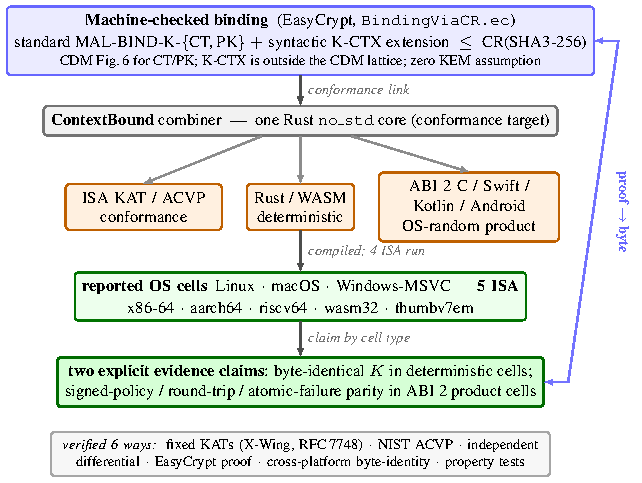
\includegraphics[width=\columnwidth]{fig_arch.pdf}
\caption{Proof-to-byte. One machine-checked binding result (top) is realized by a single Rust
\code{no\_std} core, exposed through five language faces and run across three operating systems
and five instruction-set architectures, all converging on a byte-identical shared secret~\K{}
(bottom); verified six ways.}
\label{fig:arch}
\end{figure}

\paragraph*{Contributions}
\begin{itemize}
\item \textbf{C1 (\cref{sec:kernel}).} An \emph{assumption-minimal, machine-checked}
\emph{commitment / transcript-binding} result: ContextBound's session key commits to the full
transcript, reducing \mbox{MAL-BIND-K-CT}, \mbox{-K-PK}, and a (non-standard) context extension
\mbox{-K-CTX} to collision-resistance of SHA3 \emph{alone}, with the injective encoding proved and
the Cremers--Dax--Medinger Figure-6 game discharged for both rejection styles in EasyCrypt. We are
explicit (\cref{sec:kernel}) that the cryptographic content is this injective-encoding + CR(SHA3)
argument---the component $\mathrm{Decaps}$ is \emph{inert}, which is exactly why no KEM assumption
is needed---and that C1's value is its completeness, mechanization, and role as the proven object
tied to C2, not proof difficulty.
\item \textbf{C2 (\cref{sec:substrate}).} \emph{Proof-to-byte cross-substrate equivalence}: the
same proven combiner is byte-identical across 5 language faces and 3 OSes, executed natively on
3 ISAs and cross-compiled with by-construction identity on 2 more, verified by a six-method
conformance matrix.
\item \textbf{C3 (\cref{sec:assurance}).} Reproducible assurance \emph{instruments}, configured as
CI gates: a self-validating source$\to$binary constant-time probe that \emph{discriminates} clean
(ML-KEM) from leaky (HQC) (HQC's leak is known; the contribution is the discriminating, gated
oracle); an executable \emph{regression oracle} for the known dk-format binding coupling; and two
independent symbolic provers. We report the constant-time measurements honestly as local runs.
\item \textbf{C4 (\cref{sec:eval}).} A production TLS~1.3 path (rustls \code{CryptoProvider}),
evaluated under real \code{tc netem}.
\end{itemize}

\paragraph*{What is and is not novel}
We state the boundary plainly. \emph{Not novel, and attributed:} that a ``hash-everything''
combiner is binding from collision-resistance alone while a lean combiner inherits the omitted
component's binding is the Chempat result~\cite{chempat}; ContextBound \emph{is} that
construction, not a new primitive. That ML-KEM's expanded-dk form breaks binding (and the seed
form fixes it) is Schmieg's~\cite{schmieg}. The binding-notion lattice is
CDM's~\cite{cdm}. That a constant-time harness must mark only secret sub-fields is standard
practice~\cite{kyberslash}. \emph{Novel:} the \emph{conjunction} C1$\wedge$C2---a CR-only,
machine-checked binding result whose proven object is demonstrably byte-identical across a
heterogeneous substrate, which no prior work provides; the self-validating source$\to$binary
\emph{discriminator} as a reusable CI artifact; and the operationalized design invariant that
binding the ciphertext and public key in the KDF makes hybrid binding robust to the component
KEM's key-serialization format. We do \textbf{not} claim stronger binding than X-Wing
(\cref{sec:kernel}), nor any live exploited deployment. \Cref{tab:position} makes the
conjunction concrete: the delta is that no prior effort ties a mechanized hybrid-combiner binding
theorem to a byte-identical multi-substrate realization with source$\to$binary and TLS gates---and
we are equally explicit that an axis we do \emph{not} hold (a verified specification-to-binary
implementation) is held by formosa-mlkem.

\begin{table}[t]\centering\footnotesize
\setlength{\tabcolsep}{3.2pt}\renewcommand{\arraystretch}{1.15}
\caption{Positioning. \checkmark\ holds; $\sim$ partial; blank: not provided. The contribution is
the \emph{conjunction} (last column), not any single row.}\label{tab:position}
\begin{tabular}{@{}p{3.55cm} c c c c c@{}}
\toprule
 & \rotatebox{90}{X-Wing} & \rotatebox{90}{formosa} & \rotatebox{90}{SandboxAQ} & \rotatebox{90}{Chempat} & \rotatebox{90}{\textbf{this work}} \\
\midrule
Mechanized binding (combiner)        &       &        & $\sim$ &        & \checkmark \\
Both rejection styles, $\K\neq\bot$  &       &        &        & $\sim$ & \checkmark \\
Zero KEM-binding assumption          &       &        &        & \checkmark & \checkmark \\
Byte-identical multi-substrate object&       &        &        &        & \checkmark \\
Source$\to$binary CT gate            &       & $\sim$ &        &        & \checkmark \\
Production TLS 1.3 path              & $\sim$ &        &        &        & \checkmark \\
\midrule
Verified spec$\to$binary impl.\ \emph{(we do not)} &  & \checkmark & $\sim$ & & \\
\bottomrule
\end{tabular}
\end{table}

\section{Background and Threat Model}\label{sec:bg}
\subsection{PQ/T hybrid KEMs and combiners}
ML-KEM~\cite{fips203} is the standardized form of CRYSTALS-Kyber~\cite{kyber}; like most lattice
KEMs it applies a Fujisaki--Okamoto transform~\cite{fo,hhk} with \emph{implicit rejection} (a
malformed ciphertext yields a pseudorandom key rather than $\bot$). The companion signature
standards are ML-DSA~\cite{fips204} and SLH-DSA~\cite{fips205}, and the broader process is surveyed
in~\cite{nistpqc}. Hybrid key exchange in TLS~1.3~\cite{rfc8446} follows the IETF
design~\cite{tlshybrid}---e.g.\ the \code{X25519MLKEM768} group~\cite{tlsmlkem} over
X25519~\cite{rfc7748}---and deployed PQ/T protocols include Signal's PQXDH~\cite{pqxdh} and Apple's
PQ3~\cite{pq3}.

A hybrid KEM combines component shared secrets $ss_{\mathrm{pq}}$ and $ss_{\mathrm{tr}}$ into a
session key \K. The design space ranges from simple \emph{concatenation} KDFs
(\code{X25519MLKEM768}) to combiners that additionally absorb ciphertexts and public keys.
X-Wing~\cite{xwing} uses a fixed ``lean'' combiner
$\K=\mathrm{SHA3}(ss_{\mathrm{pq}}\,\|\,ss_{\mathrm{tr}}\,\|\,ct_{\mathrm{tr}}\,\|\,pk_{\mathrm{tr}}\,\|\,\mathrm{label})$,
omitting the ML-KEM ciphertext and public key.

\subsection{KEM binding}
We use the Cremers--Dax--Medinger (CDM) \mbox{X-BIND-$P$-$Q$} framework~\cite{cdm}. A
\emph{transcript} is a tuple $(pk, ct, \K)$ produced by a (possibly malicious) execution; the two
``observable'' quantities a binding notion may constrain are the public key $\textsf{PK}$, the
ciphertext $\textsf{CT}$, and the derived key $K$. For $P,Q\in\{K,\textsf{PK},\textsf{CT}\}$, a KEM
is \mbox{X-BIND-$P$-$Q$} if no adversary in the game below wins:

\smallskip
\noindent\fbox{\parbox{0.95\columnwidth}{\footnotesize
\textbf{Game} $\mathsf{Bind}^{P,Q}_{\mathcal{A}}$: the adversary $\mathcal{A}$ outputs two
transcripts $(pk_0,ct_0,\K_0)$ and $(pk_1,ct_1,\K_1)$. $\mathcal{A}$ \emph{wins} iff
$\;P_0 = P_1\;\wedge\;Q_0 \neq Q_1\;\wedge\;\K_0\neq\bot\;\wedge\;\K_1\neq\bot$.}}
\smallskip

\noindent Three adversary classes parameterize how the key material in each transcript is produced,
in increasing strength: \textbf{HON} (honest \textsf{KeyGen}), \textbf{LEAK} (honest keys, secret
keys leaked to $\mathcal{A}$), and \textbf{MAL} (adversarially generated keys). Thus MAL~$\supseteq$~LEAK~$\supseteq$~HON,
and CDM prove monotonicity across the $(P,Q)$ lattice, so \mbox{MAL-BIND-K-CT} and
\mbox{MAL-BIND-K-PK} jointly yield the whole K-binds-$\{$PK,CT$\}$ sub-lattice. For
implicitly-rejecting KEMs such as ML-KEM, these two are the achievable ceiling on those axes; the
dual \mbox{X-BIND-CT-$\ast$} notions (a ciphertext binding the key or public key) are
\emph{structurally unachievable}, since decapsulation never returns $\bot$ and a mutated ciphertext
always yields \emph{some} key. The binding of implicitly-rejecting KEMs---and how it fails under
malicious, expanded-form keys---is studied in detail by Schmieg and others~\cite{schmieg,cdmrej}.

\subsection{Threat model}
We consider three adversaries. The \emph{malicious-key (MAL) binding} adversary supplies
adversarial keypairs and seeks colliding transcripts (\cref{sec:kernel}). The
\emph{binary-level constant-time} adversary observes secret-dependent control flow / memory
indexing in the \emph{compiled} code (\cref{sec:assurance}). The \emph{downgrade/agility}
adversary attacks profile and policy negotiation (handled by fail-closed policy binding; out of
scope here). Confidentiality of the component primitives (IND-CCA2 of ML-KEM, the
Diffie--Hellman assumption for X25519) is assumed, not re-proved.

\section{ContextBound and the Machine-Checked Kernel}\label{sec:kernel}
\subsection{Construction}
ContextBound derives
\(
\K=\mathrm{SHA3\text{-}256}\big(\mathrm{encode}[\textsf{LABEL},\textsf{suite\_id},
\textsf{policy\_version}, ss_{\mathrm{pq}}, ss_{\mathrm{tr}}, ct_{\mathrm{pq}}, pk_{\mathrm{pq}},
ct_{\mathrm{tr}}, pk_{\mathrm{tr}}, \textsf{context}]\big),
\)
where \code{encode} concatenates each field under a fixed-width 8-byte big-endian length prefix
(\cref{alg:encode}). Two design choices are load-bearing. \emph{(i) Inject\-ive, length-prefixed
encoding.} A naive concatenation $a\,\|\,b$ is ambiguous---$(\text{``}ab\text{''},\text{``''})$ and
$(\text{``}a\text{''},\text{``}b\text{''})$ collide---which is precisely the structure a binding
adversary exploits. Prefixing every field with its fixed-width length makes the encoding
self-delimiting and therefore injective (proved, \cref{sec:kernel}), so distinct transcripts map to
distinct byte strings and the binding question reduces cleanly to collision-resistance of the hash.
\emph{(ii) Absorb everything.} ContextBound feeds \emph{all} component ciphertexts and public keys
(and an application context, and a domain-separating label, suite identifier, and policy version)
into the hash. By the combiner-binding theorem of Chempat~\cite{chempat}, the binding advantage is
then bounded by $\mathrm{Adv}^{\mathrm{CR}}$ alone, with no residual term requiring any component
KEM to be binding---trading a KEM-self-binding assumption for a single, well-studied
collision-resistance assumption. The dual profile \code{CompatXWing} reproduces X-Wing's lean
combiner byte-for-byte for interoperability; \code{ContextBound} is the hash-everything profile and
is policy-selected when an application needs context binding or wishes to avoid the
serialization-format dependence of \cref{sec:assurance}. The suite is open
source.\footnote{\url{https://github.com/billlza/q-periapt}}

\begin{algorithm}[t]\small
\DontPrintSemicolon
\KwIn{label $L$, suite id $S$, version $v$, secrets $ss_{\mathrm{pq}},ss_{\mathrm{tr}}$,
ciphertexts $ct_{\mathrm{pq}},ct_{\mathrm{tr}}$, public keys $pk_{\mathrm{pq}},pk_{\mathrm{tr}}$,
context $x$}
\KwOut{32-byte shared secret \K}
$\mathsf{lp}(f) \gets \mathsf{be8}(|f|)\,\|\,f$ \tcp*{8-byte big-endian length prefix}
$T \gets [\,L,\,S,\,\mathsf{be4}(v),\,ss_{\mathrm{pq}},\,ss_{\mathrm{tr}},\,ct_{\mathrm{pq}},\,pk_{\mathrm{pq}},\,ct_{\mathrm{tr}},\,pk_{\mathrm{tr}},\,x\,]$\;
$e \gets \mathsf{lp}(T_0)\,\|\,\mathsf{lp}(T_1)\,\|\,\cdots\,\|\,\mathsf{lp}(T_{n-1})$ \tcp*{injective encode}
\Return $\mathrm{SHA3\text{-}256}(e)$\;
\caption{\textsc{ContextBound} combiner. \code{CompatXWing} omits
$ct_{\mathrm{pq}},pk_{\mathrm{pq}},S,v,x$ and uses X-Wing's label.}\label{alg:encode}
\end{algorithm}

\subsection{The EasyCrypt development}
\Cref{fig:kernel} shows the mechanized reduction. The encoding's injectivity, \code{encode\_inj},
is a \emph{proved lemma}, not an assumed one. The proof has two steps. A field-level lemma,
\code{lp\_cat\_inj}, shows that a single length-prefixed field is self-delimiting: if
$\mathsf{lp}(a)\,\|\,x = \mathsf{lp}(b)\,\|\,y$ then $a=b$ and $x=y$, because the two 8-byte
prefixes have equal width and (being injective) force $|a|=|b|$, after which list-concatenation
cancellation (\code{eqseq\_cat}) splits off equal field bodies and equal remainders. A structural
induction over the field list then lifts this to whole encodings: a non-empty encoding has size
$\ge 8$ and so can never equal the empty one, ruling out boundary-shift collisions, and the
inductive step peels one field with \code{lp\_cat\_inj}. The whole argument bottoms out at two
elementary facts about the length field---that an 8-byte big-endian integer occupies 8 bytes
(\code{be8\_size}) and is injective (\code{be8\_inj}). On top of \code{encode\_inj} we discharge (i)
a generic transcript-collision reduction \code{bind\_le\_cr}: a \code{byequiv} argument that maps any
adversary winning the binding game to one finding an $H$-collision, since a differing observable
forces a differing field list (hence, by injectivity, a differing encoding) while the colliding key
forces equal hashes; and (ii) the \emph{KEM-aware} game, in which
the MAL adversary supplies the keypairs and \K{} is \emph{derived} via the component
$\mathrm{Decaps}$ functions and the combiner. We mechanize both the implicit-rejection
specialization (\code{malbind\_*\_le\_cr}) and the fully general CDM Figure-6 game with explicit
rejection (\code{malbind\_*\_xrej\_le\_cr}), where the $\K\neq\bot$ side condition is
\emph{present and load-bearing}---removing it makes the proof fail. Every theorem reduces only to
$\mathrm{CR}(\mathrm{SHA3})$; the development compiles under the EasyCrypt checker (we pin the
checker and SMT-solver versions in the artifact), and each theorem is verified load-bearing on
\code{encode\_inj} by an adversarial negative control.

\emph{What this is, precisely.} We state the cryptographic content plainly, because a
CDM-literate reader should not over-read the label. Since \K{} \emph{is defined} as
$H(\mathrm{encode}[\dots])$ and the tuple contains the ciphertexts and public keys
\emph{directly}, the proof is in substance a \emph{commitment / transcript-binding} statement: it
shows that one cannot collide \K{} while changing a ciphertext, public key, or context, by
reducing to $\mathrm{CR}(H)$ over the proved injective encoding. The component
$\mathrm{Decaps}$---and hence the adversary's freedom over key material that CDM binding is
fundamentally about---is \emph{inert} in the argument: the theorems would hold for \emph{any}
$\mathrm{Decaps}$, which is exactly what ``zero KEM assumption'' means and why it is achievable.
The value of C1 is therefore its \emph{completeness} (both rejection styles, with $\K\neq\bot$
discharged), its \emph{mechanization}, and its role as the \emph{proven object} carried,
byte-identically, across the substrate of \cref{sec:substrate}---not proof difficulty. The
concrete attack-resistance arguments (re-encapsulation, the dk-format coupling of
\cref{sec:assurance}) are \emph{design arguments} consistent with this commitment property, not
claims the EasyCrypt artifact witnesses at the $\mathrm{Decaps}$ level.

\begin{figure}[t]\centering
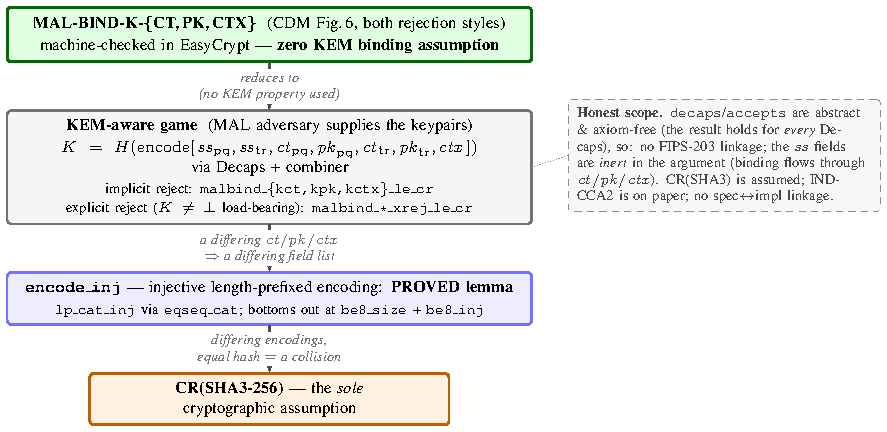
\includegraphics[width=\columnwidth]{fig_kernel.pdf}
\caption{The kernel as a reduction tower: \mbox{MAL-BIND-K-\{CT,PK,CTX\}} (CDM Figure~6, both
rejection styles) reduces---using no property of $\mathrm{Decaps}$---through the proved
\code{encode\_inj} to collision-resistance of SHA3, the sole cryptographic assumption.}
\label{fig:kernel}
\end{figure}

\subsection{Honest binding position}
\Cref{fig:binding} states our position precisely. On the standard \{CT,PK\} axes, ContextBound and
a correctly-implemented seed-dk X-Wing both reach the \mbox{MAL-BIND-K-\{CT,PK\}} ceiling; we are
\emph{not} ``stronger'' there. Our edge is (a) \emph{assumption-minimality}: ContextBound's
binding reduces to CR(SHA3) alone, whereas X-Wing's relies on ML-KEM's Fujisaki--Okamoto
self-binding together with the seed-dk format; (b) \emph{mechanization}; and (c) \emph{dk-format
robustness} (\cref{sec:assurance}). Honest scope of the mechanization: $\mathrm{Decaps}$ is
modelled as an abstract function (which is exactly why ``zero KEM assumption'' is literal), so
there is no FIPS-203 linkage and the shared-secret fields are inert in the binding argument;
CR(SHA3) is assumed; IND-CCA2 robustness is argued on paper; and there is no
specification-to-implementation linkage proof.

\begin{figure}[t]\centering
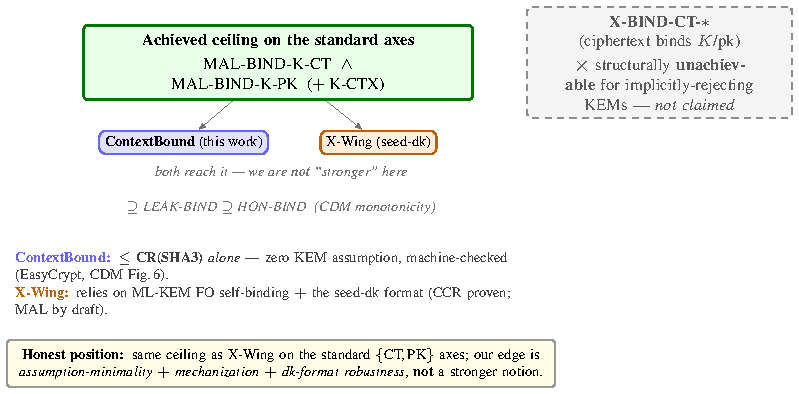
\includegraphics[width=\columnwidth]{fig_binding.pdf}
\caption{Honest binding position. Both schemes reach the standard ceiling; our edge is
assumption-minimality, mechanization, and dk-format robustness---not a stronger notion.
\mbox{X-BIND-CT-$\ast$} is structurally unachievable for implicitly-rejecting KEMs and is not
claimed.}
\label{fig:binding}
\end{figure}

\section{Proof-to-Byte Cross-Substrate Realization}\label{sec:substrate}
A single dependency-free Rust \code{no\_std} core implements the combiner and the binding/encoding
logic; vetted backends (libcrux ML-KEM, x25519-dalek, libcrux SHA3) are injected through traits.
The core is exposed through five language faces (Rust, a C ABI, WebAssembly, Swift, Kotlin).
Because the proven object is one piece of code, the question becomes whether \emph{every}
realization produces the same bytes.

\Cref{tab:verif} lists the six orthogonal methods (NIST ACVP vectors~\cite{acvp} among them) that answer this. They are deliberately
heterogeneous in their oracle and in what they catch, so a defect that escapes one is caught by
another. \Cref{tab:substrate} reports the substrate coverage with honest per-cell status: the
byte-identical shared secret is \emph{run} natively on x86-64, aarch64, and wasm32; on riscv64 and
the bare-metal \code{thumbv7em} target the core cross-compiles cleanly and byte-identity follows by
construction from the FIPS-deterministic encodings and identical source, but is not executed on a
native runner. This honest accounting is what makes the cross-substrate claim defensible.

\emph{Footprint.} The deployable surface is small: the stripped C-ABI shared library---the
\emph{entire} suite, including libcrux ML-KEM and ML-DSA---is $441$\,KB; the WebAssembly module is
$249$\,KB; and the dependency-free core cross-compiles to the bare-metal \code{thumbv7em} target, so
the same proven combiner runs from a server down to an embedded MCU.

\begin{table*}[t]\centering\footnotesize
\setlength{\tabcolsep}{6pt}\renewcommand{\arraystretch}{1.2}
\caption{The six orthogonal verification methods.}\label{tab:verif}
\begin{tabular}{@{}>{\bfseries}l p{3.4cm} p{2.6cm} p{6.6cm}@{}}
\toprule
\textbf{Method} & \textbf{Reference / oracle} & \textbf{Independence} & \textbf{What it catches} \\
\midrule
Fixed KATs & X-Wing draft vectors; RFC 7748 & published vectors & combiner and X25519 spec-conformance regressions \\
NIST ACVP & \emph{usnistgov} ACVP, full FIPS family & NIST ground truth & primitive non-conformance (FIPS 203/204/205) \\
Multi-backend differential & RustCrypto \code{ml-kem}/\code{ml-dsa}; orion X25519 & independent re-implementations & implementation bugs (output must stay byte-identical) \\
EasyCrypt proof & machine-checked; CR(SHA3) & formal (computational) & binding-design flaws in the combiner \\
Cross-platform byte-identity & shared test vector & 5 faces $\times$ substrates & per-substrate divergence (same \K{} everywhere) \\
Generative property tests & proptest: 7 properties $\times$ 128 cases & randomized & edge-case violations (injectivity, domain separation, K-CTX) \\
\bottomrule
\end{tabular}
\end{table*}

\begin{table}[t]\centering\footnotesize
\setlength{\tabcolsep}{4pt}\renewcommand{\arraystretch}{1.15}
\caption{Cross-substrate coverage (\checkmark\ verified, CI or local).}\label{tab:substrate}
\begin{tabular}{@{}l l c c c@{}}
\multicolumn{5}{@{}l}{\emph{(a) ISA targets (Rust core; the byte-level claim)}}\\
\toprule
\textbf{ISA} & \textbf{runner} & \textbf{build} & \textbf{byte-id.\ \K} & \textbf{binary-CT} \\
\midrule
x86-64 & Linux, Win-MSVC & \checkmark & \checkmark\,(run) & \checkmark\ Memcheck \\
aarch64 & Linux, macOS & \checkmark & \checkmark\,(run) & \checkmark\ Memcheck \\
wasm32 & node & \checkmark & \checkmark\,(run) & source-CT \\
riscv64 & Linux (cross) & \checkmark & by constr.$^\dagger$ & source-CT \\
thumbv7em & bare-metal & \checkmark & by constr.$^\dagger$ & n/a \\
\bottomrule
\multicolumn{5}{@{}l}{\footnotesize $^\dagger$ cross-compiled, not run natively; identity follows from}\\[-2pt]
\multicolumn{5}{@{}l}{\footnotesize \phantom{$^\dagger$} FIPS-deterministic encodings $+$ identical source.}\\[4pt]
\multicolumn{5}{@{}l}{\emph{(b) language face $\times$ OS (shared vector $\to$ same \K)}}\\
\toprule
\textbf{Face} & \textbf{Linux} & \textbf{macOS} & \textbf{Windows} & \\
\midrule
Rust & \checkmark & \checkmark & \checkmark & \\
C ABI & \checkmark & \checkmark & \checkmark\,(MSVC) & \\
WASM (node) & \checkmark & \checkmark & \checkmark & \\
Swift & \textendash & \checkmark & \textendash & \\
Kotlin (JVM/FFM) & \checkmark & \checkmark & \textendash & \\
\bottomrule
\end{tabular}
\end{table}

\section{CI-Gated Assurance}\label{sec:assurance}
\subsection{A source$\to$binary constant-time \emph{discriminator}}
libcrux proves its ML-KEM secret-independent at the \emph{source} level (a typed discipline,
machine-checked). The orthogonal \emph{binary}-level question---does the compiler reintroduce a
secret-dependent branch on the genuine secret path?---is answered by a probe that marks only the
genuinely-secret decapsulation-key sub-fields ($\hat s$, $z$) and runs the real libcrux
\code{decapsulate} under Memcheck. The probe is \emph{self-validating}: a planted secret-indexed
load is caught (harness sanity), and marking the embedded \emph{public} key flags 5696 reports
(Memcheck demonstrably sees real branches in this binary). With only the genuine secret marked,
the probe reports \textbf{zero} flags on aarch64: source-level secret-independence survives
compilation. Run against the suite's unaudited HQC backend, the same probe flags \textbf{193}
reports localized to \code{vect\_set\_random\_fixed\_weight}---so the probe is a \emph{discriminator}
(\cref{fig:ct}): clean ML-KEM versus leaky HQC in one framework. (HQC's leak is known; the
contribution is the discriminating, gated artifact and the corollary that per-backend
constant-time gating is necessary, not decorative.)

\begin{figure}[t]\centering
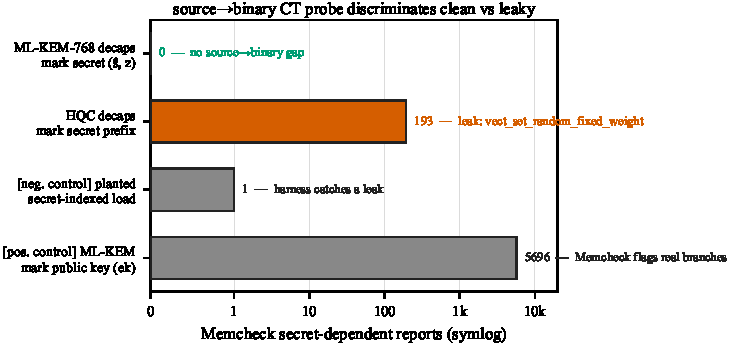
\includegraphics[width=\columnwidth]{fig_ct.pdf}
\caption{The source$\to$binary CT probe discriminates: the genuine ML-KEM secret yields zero
flags; the same harness flags HQC's constant-weight sampler (193) and validates itself with two
controls.}
\label{fig:ct}
\end{figure}

\subsection{Binding is contingent on the component dk format}
We demonstrate, executably against real libcrux, that a lean (X-Wing-shaped) combiner's
\mbox{MAL-BIND-K-PK} is \emph{contingent on} the component KEM's key-serialization format. Using
Schmieg's expanded-dk construction, two distinct ML-KEM public keys yield the same shared secret;
the lean combiner---which omits $pk_{\mathrm{pq}}$---then collides, whereas ContextBound, which
absorbs $pk_{\mathrm{pq}}$, does not. We stress that this is \emph{not} a break of X-Wing, which
mandates the seed-dk format that defeats the attack; it is a robustness separation of the combiner
\emph{shape}, and the operationalized lesson that binding ct/pk in the KDF removes a latent
dependence on the component library's serialization choice.

\subsection{Multi-prover assurance}
Beyond the computational EasyCrypt proof, the server-authenticated hybrid handshake is modelled in
two independent symbolic provers, Tamarin and ProVerif, each establishing that the session key
survives the compromise of \emph{either} component KEM. All three formal artifacts are configured as CI gates (EasyCrypt make check, Tamarin, ProVerif), with checker and solver versions pinned in the artifact.

\section{Production Integration and Evaluation}\label{sec:eval}

\subsection{Microbenchmarks}
\Cref{tab:bench} reports primitive and hybrid costs (Criterion, point estimates, on an Apple-Silicon
arm64 host; the artifact reproduces them and an x86-64 run). Two findings matter for deployment.
First, \emph{the post-quantum leg is not the bottleneck}: ML-KEM-768 encapsulation is
$11.0\,\mu$s, roughly $8\times$ cheaper than X25519 encapsulation ($89.6\,\mu$s, an ephemeral
keygen plus a Diffie--Hellman), so the classical half dominates hybrid CPU---a useful corrective to
the assumption that PQ is the expensive part. Second, \emph{the hash-everything combiner is cheap}:
ContextBound costs only $+6.2\,\mu$s over the byte-exact X-Wing combiner CompatXWing (encapsulation
$108.4$ vs.\ $102.2\,\mu$s; decapsulation $65.4$ vs.\ $59.2\,\mu$s)---the price of binding the full
transcript is sub-$10\,\mu$s, well under the $\sim$190\,$\mu$s X25519 cost and far below any network RTT.

\begin{table}[t]\centering\footnotesize
\setlength{\tabcolsep}{5pt}\renewcommand{\arraystretch}{1.15}
\caption{Primitive and hybrid cost ($\mu$s) and key/ciphertext sizes (bytes). arm64 host.}\label{tab:bench}
\begin{tabular}{@{}l r r r r r r@{}}
\toprule
 & \multicolumn{3}{c}{\textbf{time ($\mu$s)}} & \multicolumn{3}{c}{\textbf{size (B)}} \\
\cmidrule(lr){2-4}\cmidrule(lr){5-7}
\textbf{Scheme} & keygen & encaps & decaps & ek & dk & ct \\
\midrule
ML-KEM-512   & 6.6  & 6.1  & 6.8  & 800  & 1632 & 768  \\
ML-KEM-768   & 11.3 & 11.0 & 11.8 & 1184 & 2400 & 1088 \\
ML-KEM-1024  & 18.5 & 16.5 & 16.7 & 1568 & 3168 & 1568 \\
X25519       & 44.1 & 89.6 & 45.0 & 32   & 32   & 32   \\
\midrule
Hybrid, ContextBound & --- & 108.4 & 65.4 & 1216 & --- & 1120 \\
Hybrid, CompatXWing  & --- & 102.2 & 59.2 & 1216 & --- & 1120 \\
\bottomrule
\end{tabular}
\end{table}

\subsection{Handshake latency under emulated networks}
We expose ContextBound (and CompatXWing) as a TLS~1.3 key-exchange group via a rustls~\cite{rustls}
\code{CryptoProvider}, using private-use group codes; a real loopback TLS~1.3 handshake completes
over this provider. We evaluate handshake \emph{time-to-session} (TCP connect plus full TLS~1.3 handshake) over a real
loopback socket shaped by \code{tc netem}, comparing a classical X25519 baseline against the two
PQ/T profiles. \Cref{fig:netem} reports the result: the three curves coincide because latency is
RTT-dominated, and the PQ/T overhead is a \emph{fixed} cost ($\sim$190\,$\mu$s of ML-KEM CPU plus
the wire bytes of \cref{fig:wire}). At realistic RTT this is negligible: at RTT~$\ge$~20\,ms the
measured overhead is \emph{within run-to-run noise}---its sign varies across repeated runs
(\cref{fig:netem}b, error bars span two repetitions)---while the only reproducible cost is the
$\sim$190\,$\mu$s of CPU visible at RTT~0. The hybrid's $+2.27$\,KB (one ML-KEM-768 keyshare each
way) fits within the existing TLS flights and triggers no additional round-trip. The two combiner
profiles are indistinguishable: the stronger binding of the hash-everything combiner is free in
latency. We report these measurements honestly as obtained on a virtualized host; a turnkey
script reproduces the protocol on quiesced bare-metal hardware for the camera-ready (the
RTT-dominated points are already stable across repetitions).

\emph{Under jitter and loss.} Adding $3$\,ms of jitter leaves the picture unchanged (all three
groups $\approx 41$\,ms median, $\approx 50$\,ms p99.9). Under $1$--$3\%$ packet loss the median is
likewise unaffected---loss is rare relative to a handshake---but the \emph{tail} jumps to
$\sim$$1$\,s, dominated by a TCP retransmission timeout per lost packet rather than by crypto or
wire size; this RTO-driven tail falls on the classical and PQ/T handshakes alike, and at our sample
size the loss-event noise precludes a precise per-group tail comparison. The honest takeaway is
that the hybrid's extra keyshare does not \emph{systematically} worsen loss resilience: the median
is byte-insensitive and the tail is governed by transport, not by the combiner.

\begin{figure}[t]\centering
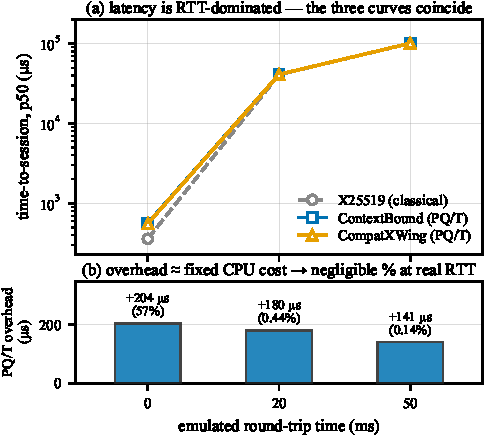
\includegraphics[width=\columnwidth]{fig_netem.pdf}
\caption{Time-to-session under real \code{tc netem} (mean of two repetitions). (a) latency is
RTT-dominated---the three curves coincide. (b) the overhead is $\sim$190\,$\mu$s of CPU at RTT~0;
at realistic RTT it is within run-to-run noise (error bars span the two repetitions and cross zero
at RTT~20\,ms).}
\label{fig:netem}
\end{figure}

\begin{figure}[t]\centering
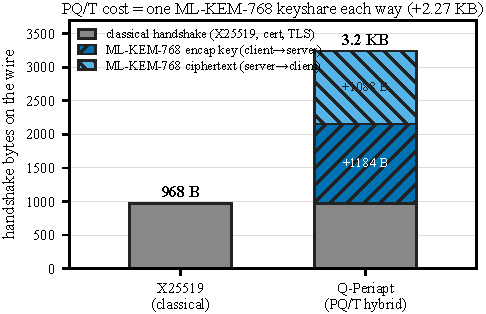
\includegraphics[width=0.86\columnwidth]{fig_wire.pdf}
\caption{Handshake wire budget. The PQ/T cost is one ML-KEM-768 keyshare each way ($+2.27$\,KB),
which fits inside the existing flights.}
\label{fig:wire}
\end{figure}

\section{Related Work}\label{sec:related}
\textbf{KEM binding.} CDM~\cite{cdm} introduced the \mbox{X-BIND-$P$-$Q$} lattice and monotonicity;
Schmieg~\cite{schmieg} proved ML-KEM's expanded-dk binding failures; Chempat~\cite{chempat}
established that hash-everything combiners are binding from collision-resistance while lean
combiners inherit the omitted component's binding (ContextBound is an instance). Context binding is
the KEM-layer analogue of context-committing AEAD~\cite{cmt}; the role of public contexts in hybrid
KEMs is analysed in~\cite{eprint2026140}. \textbf{Side channels.} KyberSlash~\cite{kyberslash} and
the ctgrind/TIMECOP discipline motivate our binary-CT gate; libcrux/HACL* provide source-level
guarantees we corroborate and discriminate against. \textbf{Hybrids in deployment.} X-Wing~\cite{xwing}
and the TLS \code{X25519MLKEM768} group are the deployed baselines we position against.
\textbf{Formal PQ.} formosa-mlkem~\cite{formosa} mechanizes ML-KEM IND-CCA; the SandboxAQ EasyCrypt-KEMs library
mechanizes \mbox{LEAK-BIND-K-PK}; our EasyCrypt~\cite{easycrypt} development adds the (commitment-style) MAL Figure-6 instantiation for the hybrid combiner, complemented by symbolic models in Tamarin~\cite{tamarin} and ProVerif~\cite{proverif}.

\section{Limitations}\label{sec:limits}
The mechanized binding result is over an \emph{abstract} $\mathrm{Decaps}$: it is exactly the
``zero KEM assumption'' that makes the result general, but it carries no FIPS-203 linkage, the
shared-secret fields are inert in the argument, and CR(SHA3) and IND-CCA2 remain assumptions argued
respectively in the model and on paper; there is no specification-to-implementation linkage proof.
Binary-level constant-time tooling is mature only on x86-64 and aarch64; riscv64 and wasm32 are
covered at source level plus upstream attestation. ACVP byte-identity is conformance, not CMVP
certification. The suite is research-grade and has not had an independent third-party audit. The
netem evaluation was obtained on a virtualized host; bare-metal reproduction is provided as a
script.

\section{Conclusion}\label{sec:concl}
A PQ/T hybrid is only as safe as its weakest realization. We closed that gap with an
assumption-minimal, machine-checked binding result whose proven object is byte-identical across a
heterogeneous deployment surface, guarded by reproducible gates (configured in CI)---a source$\to$binary
constant-time discriminator, a binding key-format coupling demonstration, and multi-prover symbolic
models---and validated on a production TLS~1.3 path. The genuinely new element is the conjunction,
not any single fact; we have been explicit about the boundary throughout.

\begin{thebibliography}{99}
\bibitem{fips203} National Institute of Standards and Technology, ``FIPS 203: Module-Lattice-Based
Key-Encapsulation Mechanism Standard,'' 2024.
\bibitem{cdm} C.~Cremers, A.~Dax, and N.~Medinger, ``Keeping Up with the KEMs: Binding Security of
Key Encapsulation Mechanisms,'' \emph{ACM CCS}, 2024. (ePrint 2023/1933.)
\bibitem{schmieg} S.~Schmieg, ``Unbindable Kemmy Schmidt: ML-KEM is neither MAL-BIND-K-CT nor
MAL-BIND-K-PK,'' IACR ePrint 2024/523, 2024.
\bibitem{chempat} J.~G\"uneysu, K.~H\"ovelmanns, \emph{et al.}, ``Binding Security of Combined KEMs
/ Chempat,'' IACR ePrint 2025/1416, 2025.
\bibitem{xwing} D.~Connolly, P.~Schwabe, and B.~Westerbaan, ``X-Wing: The Hybrid KEM You've Been
Looking For,'' draft-connolly-cfrg-xwing-kem (CFRG), 2024.
\bibitem{kyberslash} D.~J.~Bernstein, K.~Bhargavan, \emph{et al.}, ``KyberSlash: Exploiting
Secret-Dependent Division Timings in Kyber Implementations,'' \emph{IACR TCHES}, 2025.
\bibitem{cmt} M.~Bellare and V.~T.~Hoang, ``Efficient Schemes for Committing Authenticated
Encryption,'' \emph{EUROCRYPT}, 2022.
\bibitem{eprint2026140} ``On the Role of Public Contexts in Hybrid KEMs,'' IACR ePrint 2026/140.
\bibitem{fips204} National Institute of Standards and Technology, ``FIPS 204: Module-Lattice-Based
Digital Signature Standard,'' 2024.
\bibitem{fips205} National Institute of Standards and Technology, ``FIPS 205: Stateless Hash-Based
Digital Signature Standard,'' 2024.
\bibitem{kyber} J.~Bos \emph{et al.}, ``CRYSTALS-Kyber: A CCA-Secure Module-Lattice-Based KEM,''
\emph{IEEE EuroS\&P}, 2018.
\bibitem{nistpqc} G.~Alagic \emph{et al.}, ``Status Report on the Fourth Round of the NIST
Post-Quantum Cryptography Standardization Process,'' NIST IR~8545, 2025.
\bibitem{fo} E.~Fujisaki and T.~Okamoto, ``Secure Integration of Asymmetric and Symmetric
Encryption Schemes,'' \emph{CRYPTO}, 1999.
\bibitem{hhk} D.~Hofheinz, K.~H\"ovelmanns, and E.~Kiltz, ``A Modular Analysis of the
Fujisaki--Okamoto Transformation,'' \emph{TCC}, 2017.
\bibitem{rfc7748} A.~Langley, M.~Hamburg, and S.~Turner, ``Elliptic Curves for Security,'' RFC
7748, IETF, 2016.
\bibitem{rfc8446} E.~Rescorla, ``The Transport Layer Security (TLS) Protocol Version 1.3,'' RFC
8446, IETF, 2018.
\bibitem{tlshybrid} D.~Stebila, S.~Fluhrer, and S.~Gueron, ``Hybrid Key Exchange in TLS 1.3,''
draft-ietf-tls-hybrid-design, IETF, 2023.
\bibitem{tlsmlkem} K.~Kwiatkowski \emph{et al.}, ``Post-Quantum Key Exchange \code{X25519MLKEM768}
for TLS 1.3,'' draft-kwiatkowski-tls-ecdhe-mlkem, IETF, 2024.
\bibitem{pqxdh} K.~Bhargavan, C.~Jacomme, F.~Kiefer, and R.~Schmidt, ``Formal Verification of the
PQXDH Post-Quantum Key Agreement Protocol,'' \emph{IEEE S\&P}, 2024.
\bibitem{pq3} Apple Security Engineering, ``iMessage with PQ3: The New State of the Art in
Quantum-Secure Messaging,'' Apple Security Research, 2024.
\bibitem{cdmrej} K.~H\"ovelmanns \emph{et al.}, ``Binding Security of Implicitly-Rejecting KEMs and
Application to BIKE and HQC,'' IACR ePrint 2024/1233, 2024.
\bibitem{hacl} J.-K.~Zinzindohou\'e, K.~Bhargavan, J.~Protzenko, and B.~Beurdouche, ``HACL*: A
Verified Modern Cryptographic Library,'' \emph{ACM CCS}, 2017.
\bibitem{libcrux} Cryspen, ``Verified ML-KEM (Kyber) in \code{libcrux},'' 2024.
\bibitem{formosa} J.~B.~Almeida \emph{et al.}, ``Formally Verifying Kyber: Episode V,''
\emph{CRYPTO}, 2024.
\bibitem{easycrypt} G.~Barthe, B.~Gr\'egoire, S.~Heraud, and S.~Z.~B\'eguelin, ``Computer-Aided
Security Proofs for the Working Cryptographer,'' \emph{CRYPTO}, 2011.
\bibitem{tamarin} S.~Meier, B.~Schmidt, C.~Cremers, and D.~Basin, ``The TAMARIN Prover for the
Symbolic Analysis of Security Protocols,'' \emph{CAV}, 2013.
\bibitem{proverif} B.~Blanchet, ``Modeling and Verifying Security Protocols with the Applied Pi
Calculus and ProVerif,'' \emph{Found.\ Trends Priv.\ Secur.}, 2016.
\bibitem{dudect} O.~Reparaz, J.~Balasch, and I.~Verbauwhede, ``Dude, is My Code Constant Time?''
\emph{DATE}, 2017.
\bibitem{valgrind} N.~Nethercote and J.~Seward, ``Valgrind: A Framework for Heavyweight Dynamic
Binary Instrumentation,'' \emph{ACM PLDI}, 2007.
\bibitem{ctgrind} A.~Langley, ``ctgrind: Checking that Functions are Constant Time with Valgrind,''
2010.
\bibitem{acvp} National Institute of Standards and Technology, ``Automated Cryptographic Validation
Protocol (ACVP),'' \url{https://github.com/usnistgov/ACVP}, 2024.
\bibitem{rustls} J.~Birr-Pixton \emph{et al.}, ``rustls: A Modern TLS Library in Rust,''
\url{https://github.com/rustls/rustls}, 2024.
\end{thebibliography}

\appendices
\section{Artifact Availability}
The complete suite---Rust core and backends, the five language faces, the EasyCrypt/Tamarin/ProVerif
developments, the constant-time and netem harnesses, and the figure-generation
scripts---is open source at \url{https://github.com/billlza/q-periapt}. All numbers in this paper
are reproducible from that repository; the bare-metal netem protocol is provided as a script.

\section*{Acknowledgment}
The author thanks the maintainers of libcrux/HACL*, EasyCrypt, Tamarin, and ProVerif, whose tools
this work builds upon. \emph{[Funding/advisor acknowledgments to be added.]}

\end{document}
